\documentclass{article}
\usepackage[utf8]{inputenc}
\usepackage[T1]{fontenc}
\usepackage{xcolor}
\usepackage{xcolor}
\usepackage{colortbl}
\usepackage{amsmath}
\usepackage{amssymb}
\usepackage{xcolor}
\usepackage{tikz}
\usepackage[tikz]{bclogo}
\usepackage{pgfplots}
\pgfplotsset{width=1.0\columnwidth}

\begin{document}

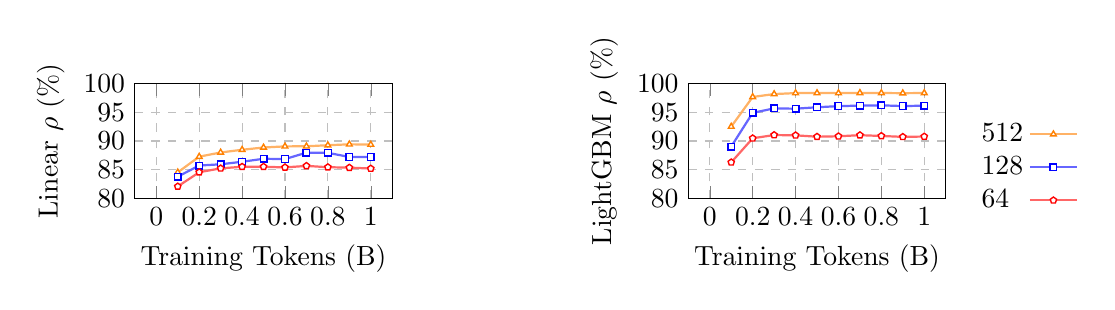
\begin{tikzpicture}
\begin{axis}[
at={(0em,0)},
width=.4\textwidth, height=.25\textwidth ,
xtick={0,0.2,...,1.0},
ytick={80, 85, ..., 105},
grid style=dashed,
ylabel={Linear $\rho$ (\%)},
xlabel={{Training Tokens (B)}},
xlabel style={align=center,yshift=0em},
ylabel style={yshift=0},
y tick style={opacity=0},
ymajorgrids=true,
xmajorgrids=true,
tick align=inside,
legend pos=outer north east,
yticklabel style={/pgf/number format/precision=0,/pgf/number format/fixed zerofill},
legend style={yshift=-0.5em,xshift=-9.7em,legend cell align=left,legend plot pos=right,draw=none},
xmin=-0.1,
xmax=1.1,
ymin=80.0,
ymax=100.0]

      \addplot[
        orange!60,mark=triangle*,mark size=1.2pt,thick,mark options={fill=white,draw=orange,line width=0.5pt}
        ]
        coordinates {
(0.1, 84.50739585717554)
(0.2, 87.25852597848477)
(0.3, 87.98917086289767)
(0.4, 88.46639677271683)
(0.5, 88.8603656443122)
(0.6, 89.05749313344012)
(0.7, 89.07301441977567)
(0.8, 89.2625600823987)
(0.9, 89.41834515907529)
(1.0, 89.3780041199359)
        };
      \addplot[
        blue!60,mark=square*,mark size=1.2pt,thick,mark options={fill=white,draw=blue,line width=0.5pt}
        ]
        coordinates {
(0.1, 83.76115815976193)
(0.2, 85.70146200503547)
(0.3, 85.92047665369648)
(0.4, 86.36615930418859)
(0.5, 86.88737411306934)
(0.6, 86.83294232089722)
(0.7, 87.96270599679559)
(0.8, 87.92558365758755)
(0.9, 87.2059538796063)
(1.0, 87.21818493934538)
        };
    \addplot[
        red!60,mark=pentagon*,mark size=1.2pt,thick,mark options={fill=white,draw=red,line width=0.5pt}
        ]
        coordinates {
(0.1, 82.03436140993362)
(0.2, 84.5289253833829)
(0.3, 85.20606832227053)
(0.4, 85.48960002288852)
(0.5, 85.48995765621422)
(0.6, 85.37587262531471)
(0.7, 85.63994907301439)
(0.8, 85.40898947127488)
(0.9, 85.33631837949186)
(1.0, 85.17452506294345)
        };
\end{axis}
\begin{axis}[
at={(20em,0)},
width=.4\textwidth, height=.25\textwidth ,
xtick={0,0.2,...,1.0},
ytick={80, 85, ..., 105},
grid style=dashed,
ylabel={LightGBM $\rho$ (\%)},
xlabel={{Training Tokens (B)}},
xlabel style={align=center,yshift=0em},
ylabel style={yshift=0},
y tick style={opacity=0},
ymajorgrids=true,
xmajorgrids=true,
tick align=inside,
legend pos=outer north east,
yticklabel style={/pgf/number format/precision=0,/pgf/number format/fixed zerofill},
legend style={yshift=-1.0em,xshift=0.5em,legend cell align=left,legend plot pos=right,draw=none},
xmin=-0.1,
xmax=1.1,
ymin=80,
ymax=100]
% (0.0, 0.0)
      \addplot[
        orange!60,mark=triangle*,mark size=1.2pt,thick,mark options={fill=white,draw=orange,line width=0.5pt}
        ]
        coordinates {
(0.1, 92.5231746395056)
(0.2, 97.71550984206911)
(0.3, 98.22535191119248)
(0.4, 98.39100766765847)
(0.5, 98.39830338750286)
(0.6, 98.39050698100249)
(0.7, 98.42104886701762)
(0.8, 98.40695811398487)
(0.9, 98.37613012130923)
(1.0, 98.40960460059507)
        };
      \addplot[
        blue!60,mark=square*,mark size=1.2pt,thick,mark options={fill=white,draw=blue,line width=0.5pt}
        ]
        coordinates {
(0.1, 89.02838178072784)
(0.2, 94.935983634699)
(0.3, 95.712405584802)
(0.4, 95.66004806591896)
(0.5, 95.91268024719614)
(0.6, 96.11080910963605)
(0.7, 96.19771400778208)
(0.8, 96.24749656672006)
(0.9, 96.1234865178486)
(1.0, 96.18727111467155)
        };
    \addplot[
        red!60,mark=pentagon*,mark size=1.2pt,thick,mark options={fill=white,draw=red,line width=0.5pt}
        ]
        coordinates {
(0.1, 86.26339159912636)
(0.2, 90.47847422125)
(0.3, 91.04610683661835)
(0.4, 90.99587559002012)
(0.5, 90.75215395088516)
(0.6, 90.82915943331062)
(0.7, 91.02118619821466)
(0.8, 90.88363390053959)
(0.9, 90.72496478655565)
(1.0, 90.78300240329592)
        };
        \legend{{512},{128},{64}}
\end{axis}
\end{tikzpicture}

\end{document}